\documentclass[table]{beamer}

\usepackage{xcolor}
\usepackage[utf8]{inputenc}
\usepackage[english,serbian]{babel}
\usepackage{graphicx}
\usetheme{Antibes}
\usecolortheme{beaver}
%Information to be included in the title page:


\title[LSTM neuronske mreže]{\textbf{LSTM neuronske mreže}}
\subtitle{primena nad problemom sekvencijalnog učenja}
\author{Nevena Soldat i Milena Kurtić}
\institute{Matematički fakultet, Univerzitet u Beogradu}
\date{\today}

\begin{document}


\frame{\titlepage}


\begin{frame}{Pregled}

\begin{itemize}
    \item Uvod
    \item Rekurentne neuronske mreže
    \item Problem generisanja teksta
    \item Rezultati
    \item Dalji razvoj
\end{itemize}

\end{frame}


\begin{frame}{Uvod}

Neuronske mreže:

\begin{itemize}
    \item jedna od najprimenjenijih metoda mašinskog učenja
    \item različite vrste (potpuno povezane, konvolutivne, rekurentne...)
    \item simulacija velike količine povezanih nervnih ćelija
\end{itemize}

\end{frame}

\begin{frame}{Opis rada}
\begin{itemize}
    \item Implementacija LSTM neuronske mreže i primena na problem generisanja teksta
    \item Baza - opisi filmova
    \item Cilj: za ulaznu sekvencu reči pretpostaviti koje će biti naredne
\end{itemize}
    
\end{frame}

\begin{frame}{Rekurentne neuronske mreže}

\begin{itemize}
\item Rekurentne neuronske mreže (eng. Recurrent Neural Network - RNN) - arhitektura neuronskih mreža specijalizovana za obradu sekvencijalnih podataka
\item Sekvence nameću važnost redosleda zapažanja podataka
\item Elementi ulazne sekvence se obrađuju u koracima
\item Mreža ima skriveno stanje koje akumulira informaciju o elementima sekvence obrađenim u prethodnim koracima
\end{itemize}
    
\end{frame}

\begin{frame}{Arhitektura RNN}
\begin{figure}[htp]
    \centering
    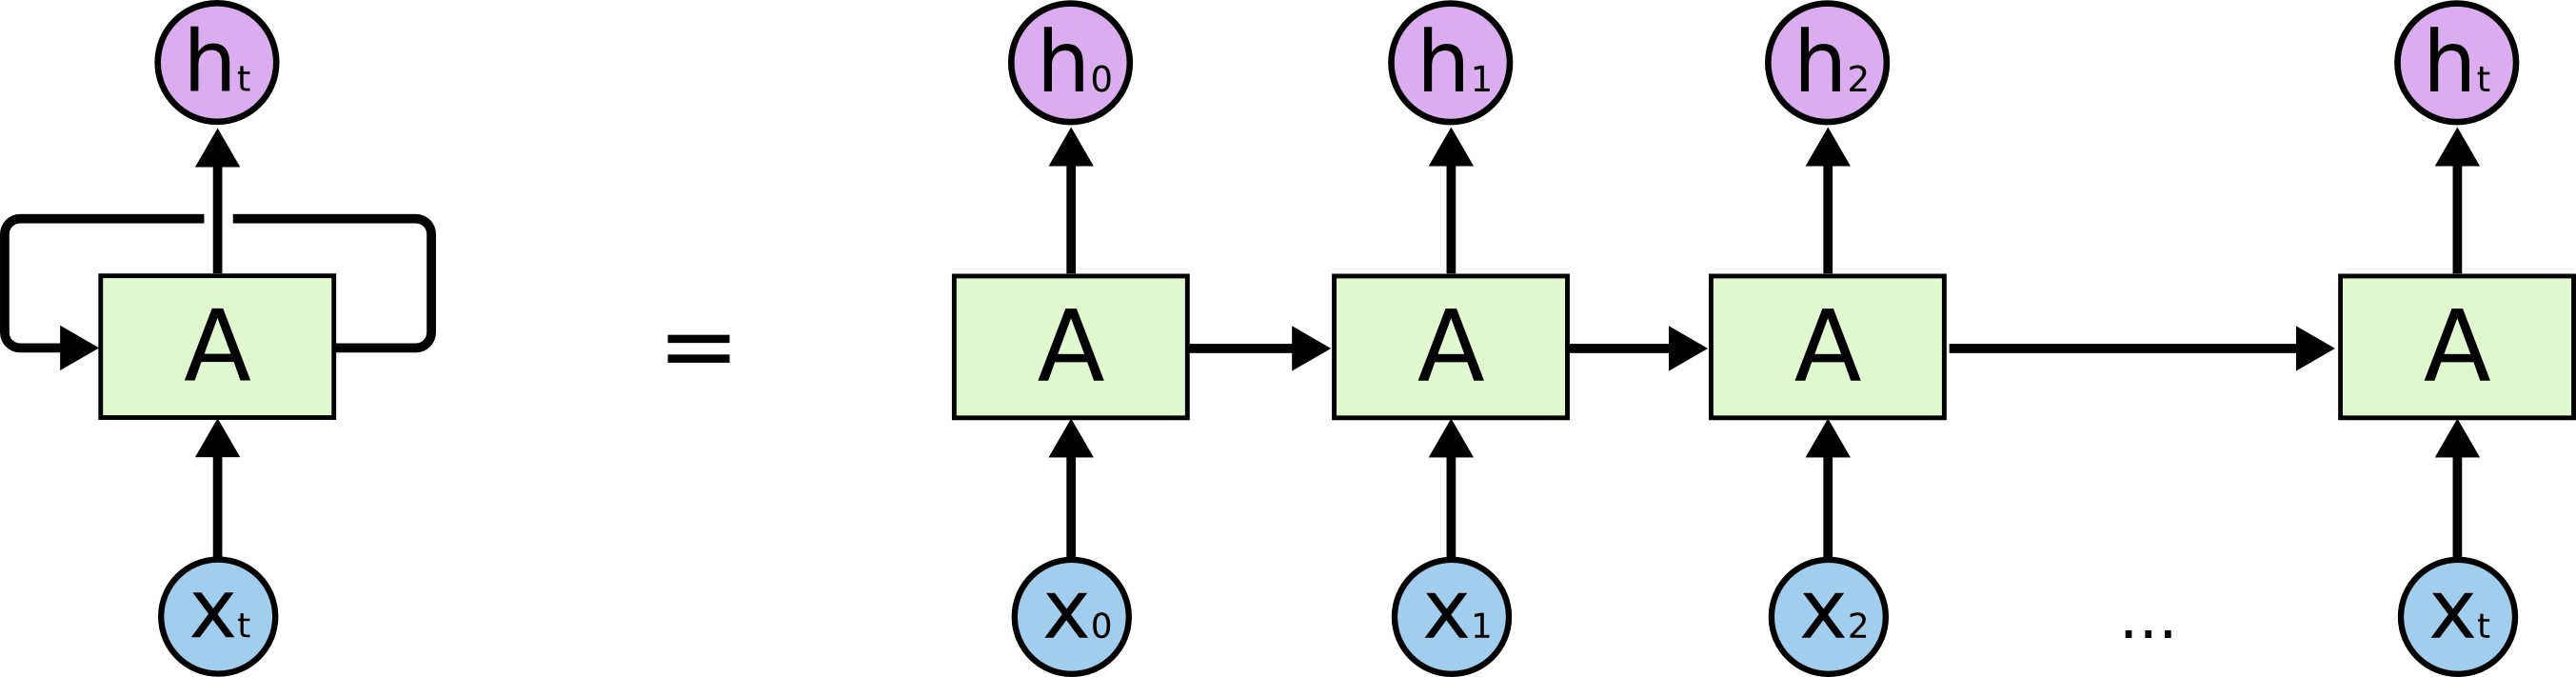
\includegraphics[scale=0.3]{RNN-unrolled.png}
\end{figure}
    
\end{frame}

\begin{frame}{Problemi sa RNN}

\begin{enumerate}
    \item \alert{Koordinate gradijenta eksplodiraju ili nestanu} prilikom izračunavanja gradijenta propagacijom u prošlost zbog velikog broja množenja
    \item \alert{Dugoročno čuvanje relevantnih informacija nije moguće} - doprinos starijih ulaza se brzo gubi pod uticajem novih. 
\end{enumerate}

\end{frame}

\begin{frame}{LSTM neuronske mreže}

\begin{itemize}
    \item duga kratkoročna memorija (eng. Long Short-Term Memory - LSTM)
    \item podvrsta rekurentnih neuronskih mreža
    \item rešavaju oba prethodno navedena problema
    \item pamćenje dugih sekvenci je praktično njihovo podrazumevano ponašanje
    \item osnovna ideja - postojanje ćelije koja čuva skriveno stanje, uz kontrolu pisanja, čitanja i zaboravljanja
\end{itemize}
    
\end{frame}

\begin{frame}{Arhitektura LSTM}
\begin{figure}
    \centering
    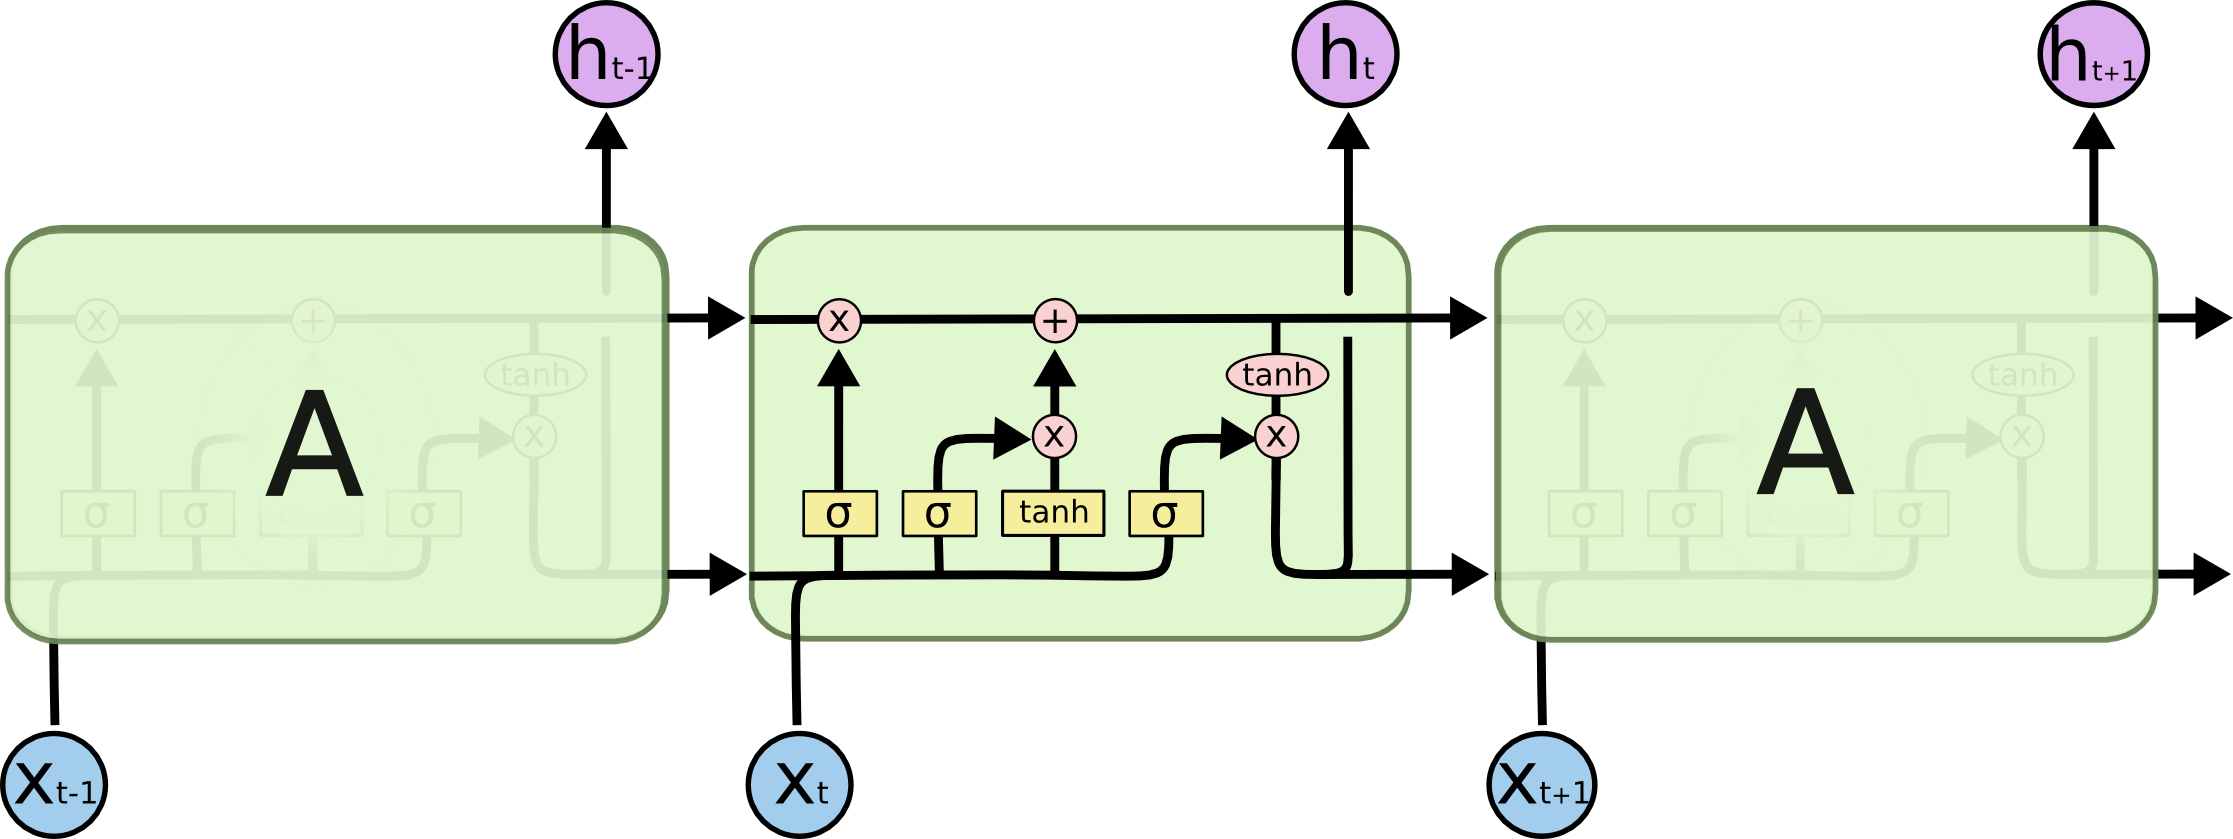
\includegraphics[scale = 0.3]{LSTM3-chain.png}
\end{figure}
    
\end{frame}

\begin{frame}{Problem generisanja teksta}
\begin{itemize}
    \item Generisanje teksta ima brojne primene, kao što su automatsko prevođenje jezika, sumarizacija teksta, generisanje opisa...
    \item Naš cilj je da dobijemo kratak opis filma, uz zadavanje ulaznih reči.
    \item Faze rešavanja:
    \begin{enumerate}
        \item Preprocesiranje teksta
        \item Kreiranje i treniranje modela
        \item Rezultati
    \end{enumerate}
\end{itemize}
    
\end{frame}


\begin{frame}{Preprocesiranje teksta}
\begin{itemize}
    \item Neuronske mreže ne mogu da rade sa sirovim podacima, odnosno tekstom
    \item Kodiramo reči kao brojeve uz pomoć Tokenizer API-a
    \item Proces tokenizacije: 
    \begin{itemize}
        \item konvertovanje svih slova u mala
        \item uklanjanje belina
        \item uklanjanje znakova interpunkcije
        \item ...
    \end{itemize}
    \item \alert{Token} - jedna reč kodirana kao broj
\end{itemize}
\end{frame}

\begin{frame}{Preprocesiranje teksta}
\begin{itemize}
    \item maksimalan broj reči - 10 000
    \item rečnik sa odgovarajućim vrednostima - {\color{orange}reč} : {\color{blue}broj}
    \item inverzni rečnik za dekodiranje - {\color{orange}broj} : {\color{blue}reč}
\end{itemize}
\begin{figure}
    \centering
    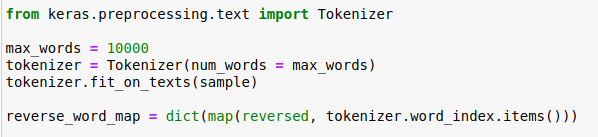
\includegraphics[scale = 0.7]{tokens.png}
\end{figure}

\end{frame}

\begin{frame}{Kreiranje ulaza i izlaza}
\begin{itemize}
    \item Biramo nasumično {\color{blue}100} filmova
    \item Uzimamo po {\color{blue}200} reči iz svakog opisa
    \item Sve opise spajamo u jedan \alert{korpus}
    \item Broj reči u korpusu - {\color{blue} 20 000}
    \item Broj različitih reči (veličina rečnika) - {\color{blue} 7003}
    \item Ulaz - sekvenca od {\color{blue} 20} reči
    \item Izlaz - naredna reč
\end{itemize}
    
\end{frame}

\begin{frame}{Primer}

\begin{itemize}
    \item Kreiranja ulaza i izlaza od sledeće rečenice: The man is walking down the street
\end{itemize}
\begin{figure}
    \centering
    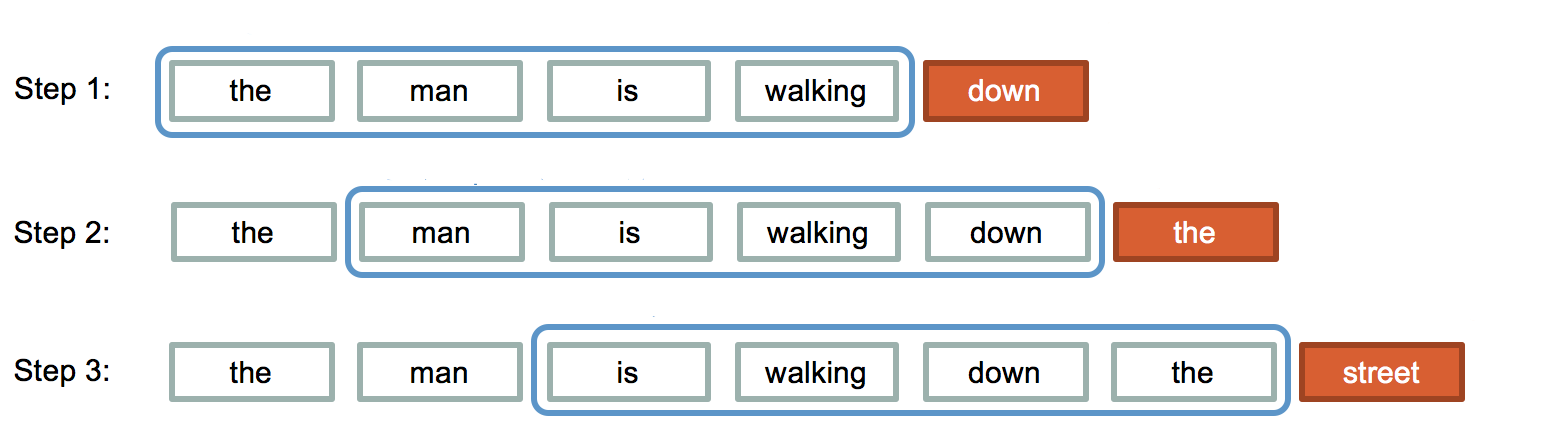
\includegraphics[scale = 0.2]{text_seq.png}
\end{figure}
\end{frame}

\begin{frame}{Arhitektura mreže}

Mreža za rešavanje problema sastoji se od narednih slojeva:
\begin{enumerate}
    \item Ulazni sloj 
    \item Prvi LSTM sloj
    \item Sloj izbacivanja 
    \item Drugi LSTM sloj
    \item Izlazni sloj
\end{enumerate}
    
\end{frame}

\begin{frame}{Arhitektura mreže}
\begin{figure}
    \centering
    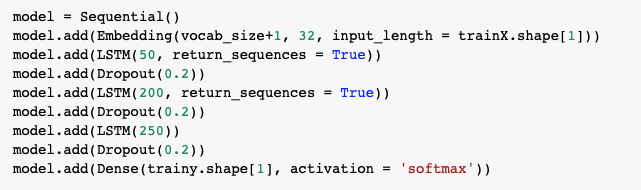
\includegraphics[scale = 0.7]{mreza.png}
\end{figure}
    
\end{frame}

\begin{frame}{Arhitektura mreže}
    \begin{figure}
        \centering
        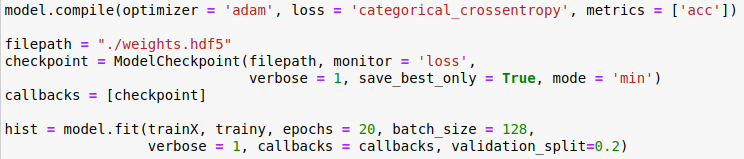
\includegraphics[scale = 0.6]{model.png}
    \end{figure}
\end{frame}

\begin{frame}{Rezultati: Brzina konvergencije}
\begin{itemize}
    \item rezultat kroz 20 epoha
\end{itemize}
\begin{figure}
    \centering
    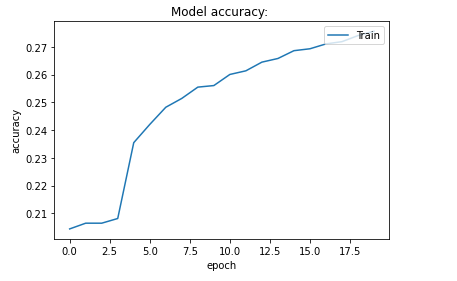
\includegraphics[scale = 0.6]{konv_20e100n.png}
\end{figure}
    
\end{frame}

\begin{frame}{Rezultati: Brzina konvergencije}
\begin{itemize}
    \item rezultat kroz 50 epoha
\end{itemize}
\begin{figure}
    \centering
    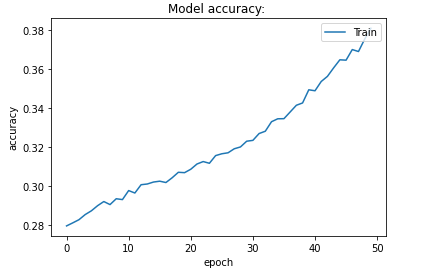
\includegraphics[scale = 0.6]{konv_50e100n.png}
\end{figure}
    
\end{frame}

\begin{frame}{Rezultati: Brzina konvergencije}
\begin{itemize}
    \item rezultat kroz 100 epoha
\end{itemize}
\begin{figure}
    \centering
    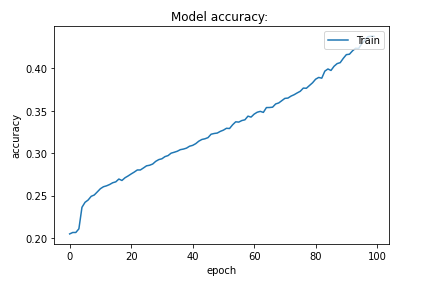
\includegraphics[scale = 0.6]{konv_100e100n.png}
\end{figure}
    
\end{frame}


\begin{frame}{Rezultati: Preciznost i greška}
\begin{table}[]
 
    \begin{tabular}{|| c c c c ||}
    \hline
    \rowcolor{lightgray!50}Broj epoha & Broj neurona & Preciznost & Gubitak \\
    \hline\hline
    \rowcolor{orange!50} 20 & 100 & 27.38 & 5.11 \\
    \rowcolor{orange!70} 50 & 100 & 38.18  & 4.27 \\
    \rowcolor{orange}100 & 100 & 43.88 & 3.88 \\
    \rowcolor{orange!50}20 & 200 & 27.80 & 4.83 \\
    \rowcolor{orange!70} 50 & 200 & 38.78 & 3.96 \\
     \hline
    \end{tabular}
    
\end{table}
\end{frame}

\begin{frame}{Rezultati: Izlaz}
\begin{itemize}
    \item rezultat kroz 20 epoha
\end{itemize}
\begin{figure}
    \centering
    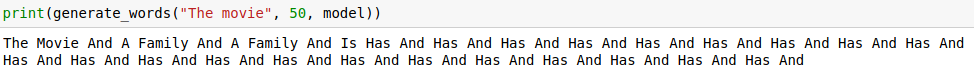
\includegraphics[scale = 0.3]{tekst_20e100n.png}
\end{figure}

\end{frame}


\begin{frame}{Rezultati: Izlaz}
\begin{itemize}
    \item rezultat kroz 50 epoha
\end{itemize}
\begin{figure}
    \centering
    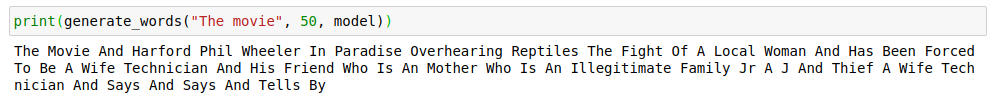
\includegraphics[scale = 0.3]{tekst_50e100n.png}
\end{figure}

\end{frame}

\begin{frame}{Rezultati: Izlaz}
\begin{itemize}
    \item rezultat kroz 100 epoha
\end{itemize}
\begin{figure}
    \centering
    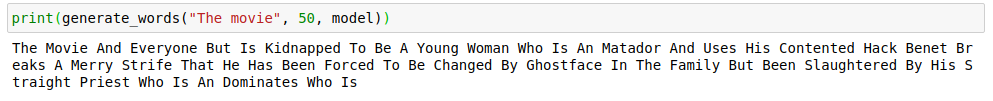
\includegraphics[scale = 0.3]{tekst_100e100n.png}
\end{figure}
    
\end{frame}

\begin{frame}{Dalji razvoj}
    \begin{itemize}
        \item povećanje broja epoha na više stotina
        \item eksperimentisanje sa brojem neurona i brojem slojeva mreže
        \item korišćenje GPU
        \item smanjenje broja ciljnih reči
        \item ...
    \end{itemize}
\end{frame}

\begin{frame}
\centering
\Large
\textbf{\alert{HVALA NA PAŽNJI!}}

\end{frame}

\end{document} 

